% Created 2025-03-17 lun 12:47
% Intended LaTeX compiler: pdflatex
\documentclass[aspectratio=169, usenames,svgnames,dvipsnames]{beamer}
\usepackage[utf8]{inputenc}
\usepackage[T1]{fontenc}
\usepackage{graphicx}
\usepackage{grffile}
\usepackage{longtable}
\usepackage{wrapfig}
\usepackage{rotating}
\usepackage[normalem]{ulem}
\usepackage{amsmath}
\usepackage{textcomp}
\usepackage{amssymb}
\usepackage{capt-of}
\usepackage{hyperref}
\usepackage{color}
\usepackage{listings}
\usepackage{mathpazo}

\usepackage[spanish]{babel}
\usepackage[symbol, perpage]{footmisc}

\usepackage{gensymb}
\usepackage{amsmath}
\usepackage{diffcoeff}
\usepackage{steinmetz}
\usepackage{mathtools}
\usepackage[output-complex-root = j]{siunitx}
\sisetup{output-decimal-marker={,}}
\DeclareSIUnit{\watthour}{Wh}

\newcommand{\laplace}[1]{\mathbf{#1}(\mathbf{s})}
\newcommand{\slp}{\mathbf{s}}
\newcommand{\fasor}[1]{\mathbf{#1}(\omega)}
\newcommand{\atan}{\mathrm{atan}}

\bibliographystyle{plain}

% https://latexcolor.com/
\definecolor{burgundy}{rgb}{0.5, 0.0, 0.13}
\definecolor{darkolivegreen}{rgb}{0.33, 0.42, 0.18}
\definecolor{frenchblue}{rgb}{0.0, 0.45, 0.73}

\usetheme{Boadilla}
\usecolortheme{rose}
\usefonttheme{serif}

\setbeamercolor{alerted text}{fg=blue!50!black} \setbeamerfont{alerted text}{series=\bfseries}

\AtBeginSubsection[]{\begin{frame}[plain]\tableofcontents[currentsubsection,sectionstyle=show/shaded,subsectionstyle=show/shaded/hide]\end{frame}}

\AtBeginSection[]{\begin{frame}[plain]\tableofcontents[currentsection,hideallsubsections]\end{frame}}
\hypersetup{colorlinks=true, linkcolor=Blue, urlcolor=Blue}

\beamertemplatenavigationsymbolsempty
\setbeamertemplate{footline}[frame number]
\setbeamertemplate{itemize items}[triangle]
\setbeamertemplate{enumerate items}[circle]
\setbeamertemplate{section in toc}[circle]
\setbeamertemplate{subsection in toc}[circle]
\parskip=5pt

\usepackage{booktabs}
\addtolength\belowrulesep{5pt}

\usetheme{default}
\author{Oscar Perpiñán Lamigueiro}
\date{}
\title{Corriente alterna sinusoidal}
\subtitle{Teoría de Circuitos}
\hypersetup{
 pdfauthor={Oscar Perpiñán Lamigueiro},
 pdftitle={Corriente alterna sinusoidal},
 pdfkeywords={},
 pdfsubject={},
 pdfcreator={Emacs 29.4 (Org mode 9.4.6)}, 
 pdflang={Spanish}}
\begin{document}

\maketitle

\section{Formas de Onda}
\label{sec:org3bfdca8}

\begin{frame}[label={sec:org59a38b7}]{Forma de Onda}
\begin{itemize}
\item La salida de los generadores (de tensión o de corriente) son funciones que pueden variar con el tiempo.
\item La dependencia funcional \(u = u(t)\) o \(i = i(t)\) se denomina forma de onda.
\end{itemize}

\begin{columns}
\begin{column}{0.3\columnwidth}
\begin{center}
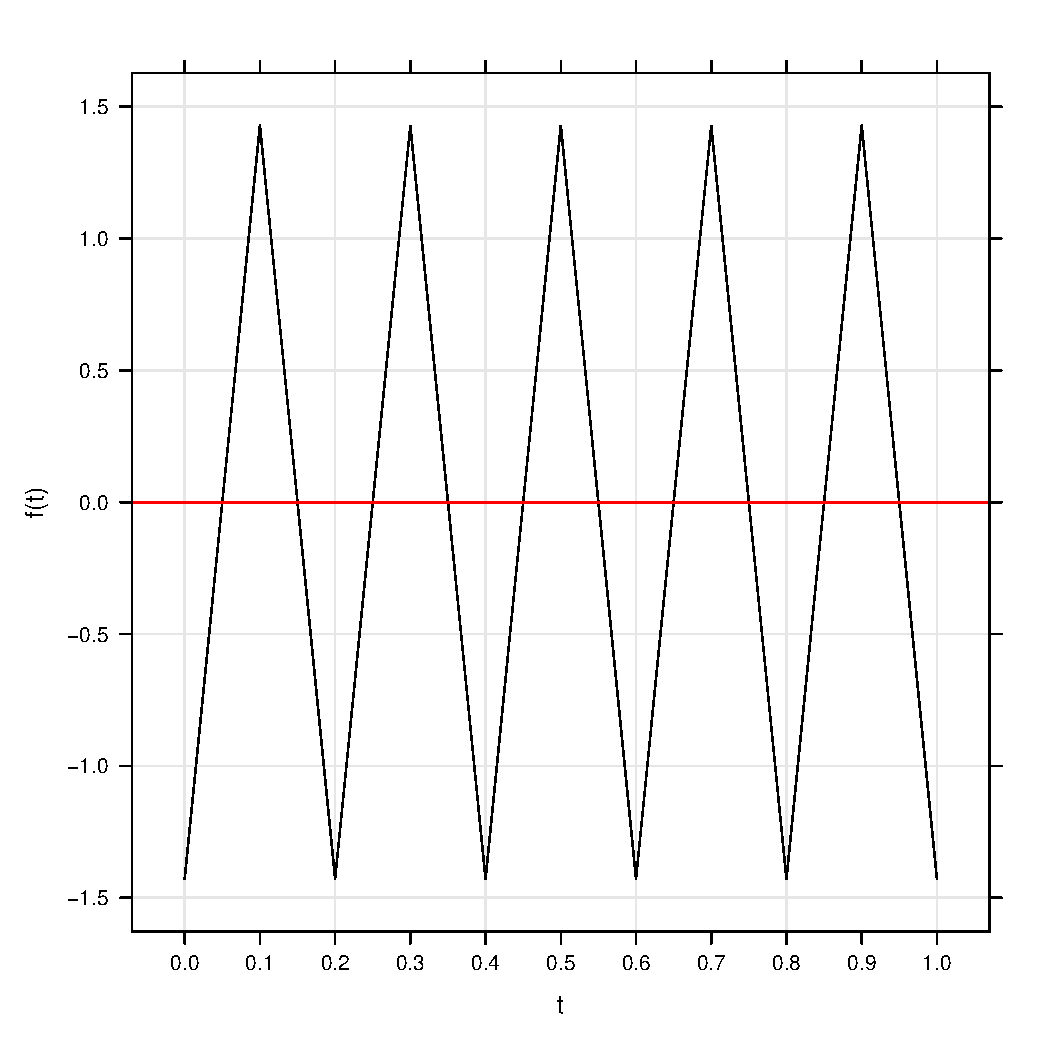
\includegraphics[width=.9\linewidth]{../figs/triangular_periodica.pdf}
\end{center}
\end{column}

\begin{column}{0.3\columnwidth}
\begin{center}
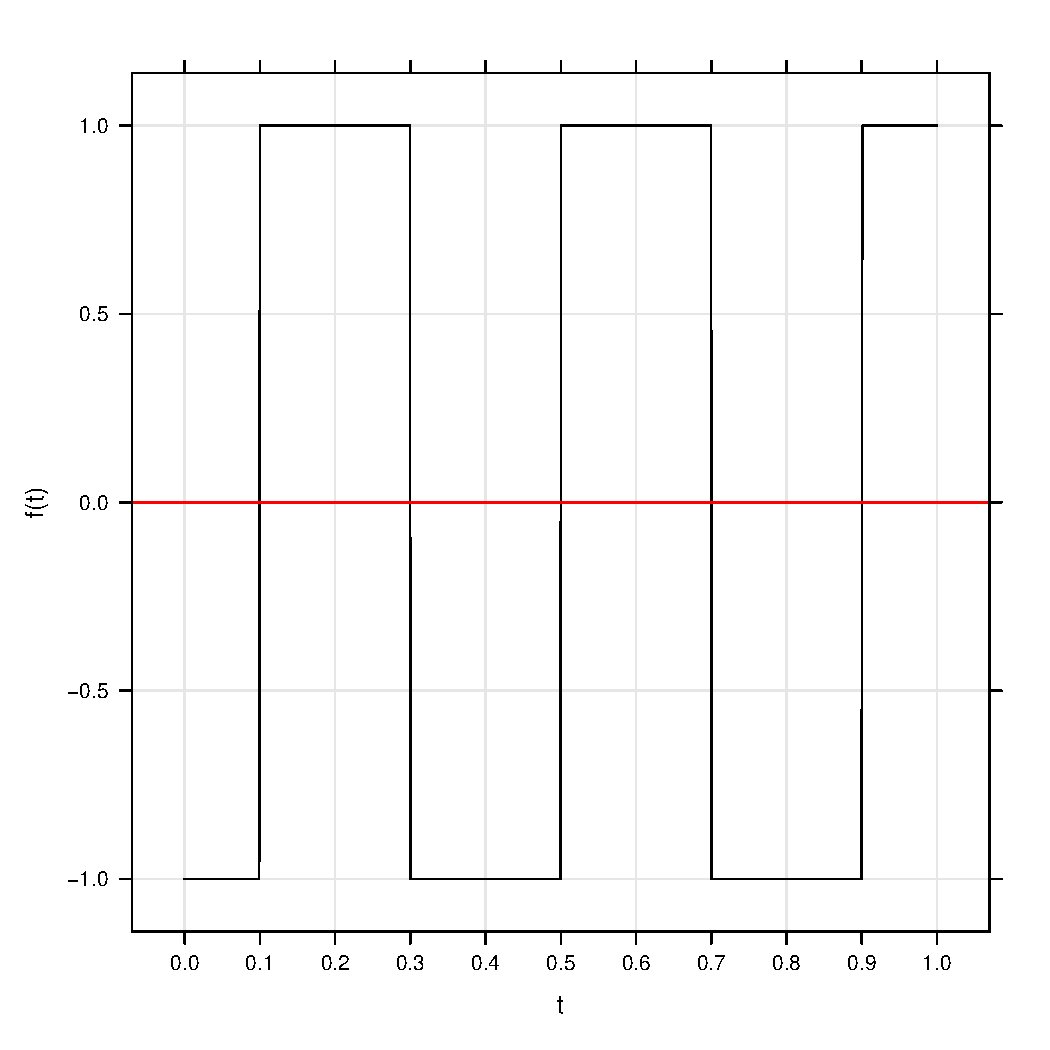
\includegraphics[width=.9\linewidth]{../figs/cuadrada_periodica.pdf}
\end{center}
\end{column}

\begin{column}{0.3\columnwidth}
\begin{center}
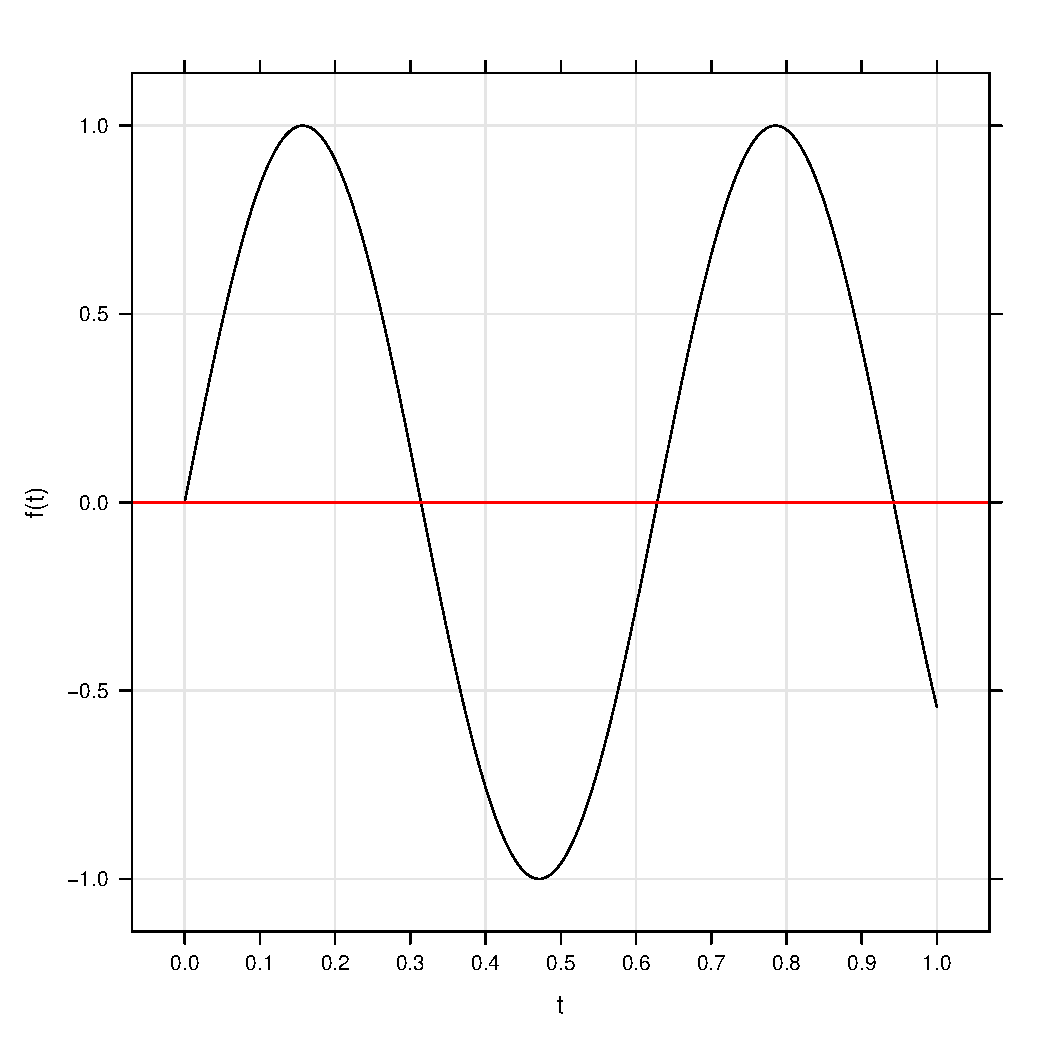
\includegraphics[width=.9\linewidth]{../figs/sin_periodica.pdf}
\end{center}
\end{column}
\end{columns}
\end{frame}

\begin{frame}[label={sec:orgd7934e1}]{Clasificación}
\begin{block}{Signo de la magnitud}
\begin{itemize}
\item Unidireccionales
\begin{itemize}
\item Signo constante
\item El valor puede ser constante (corriente continua) o variable.
\end{itemize}
\item Bidireccionales
\begin{itemize}
\item Signo variable con el tiempo.
\end{itemize}
\end{itemize}
\end{block}

\begin{columns}
\begin{column}{0.5\columnwidth}
\begin{center}
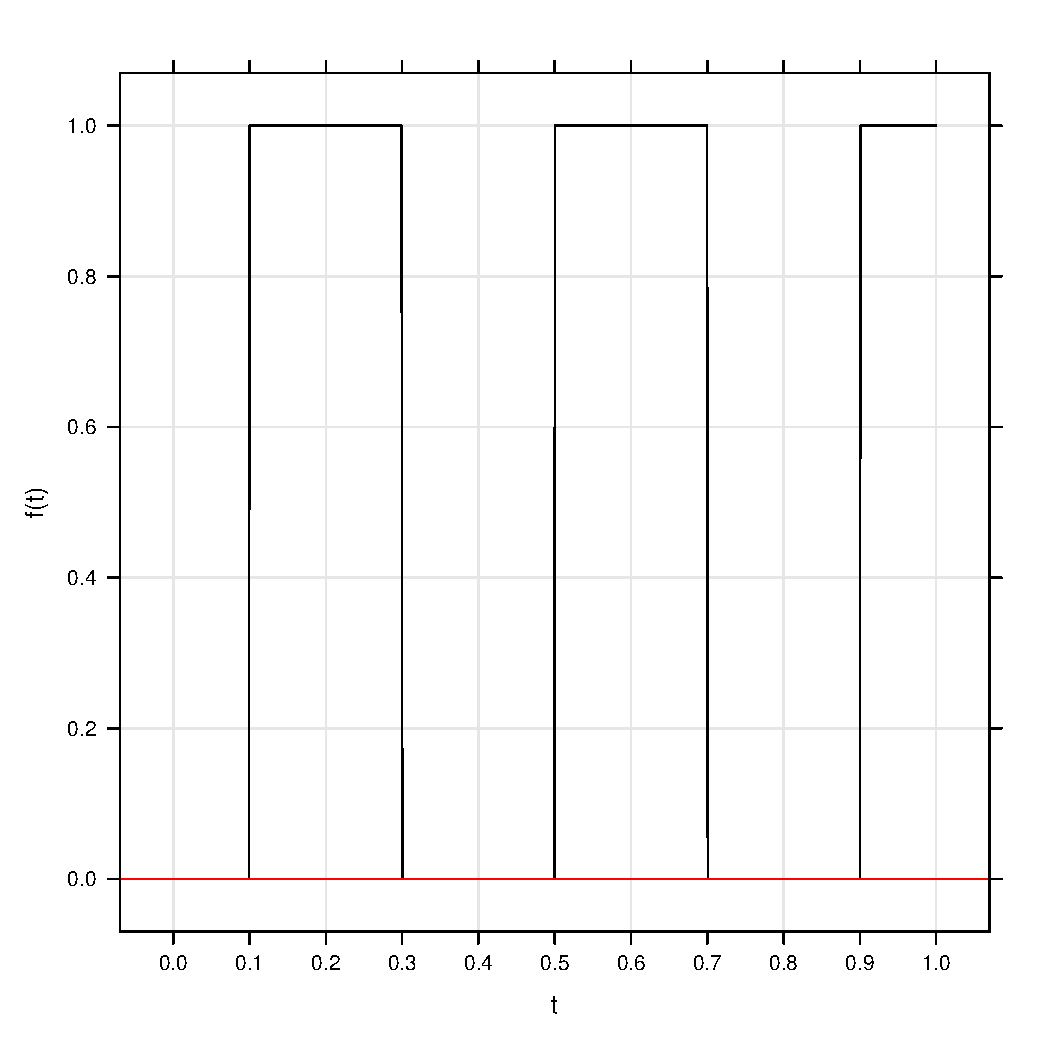
\includegraphics[height=0.52\textheight]{../figs/cuadrada0_periodica.pdf}
\end{center}
\end{column}

\begin{column}{0.5\columnwidth}
\begin{center}
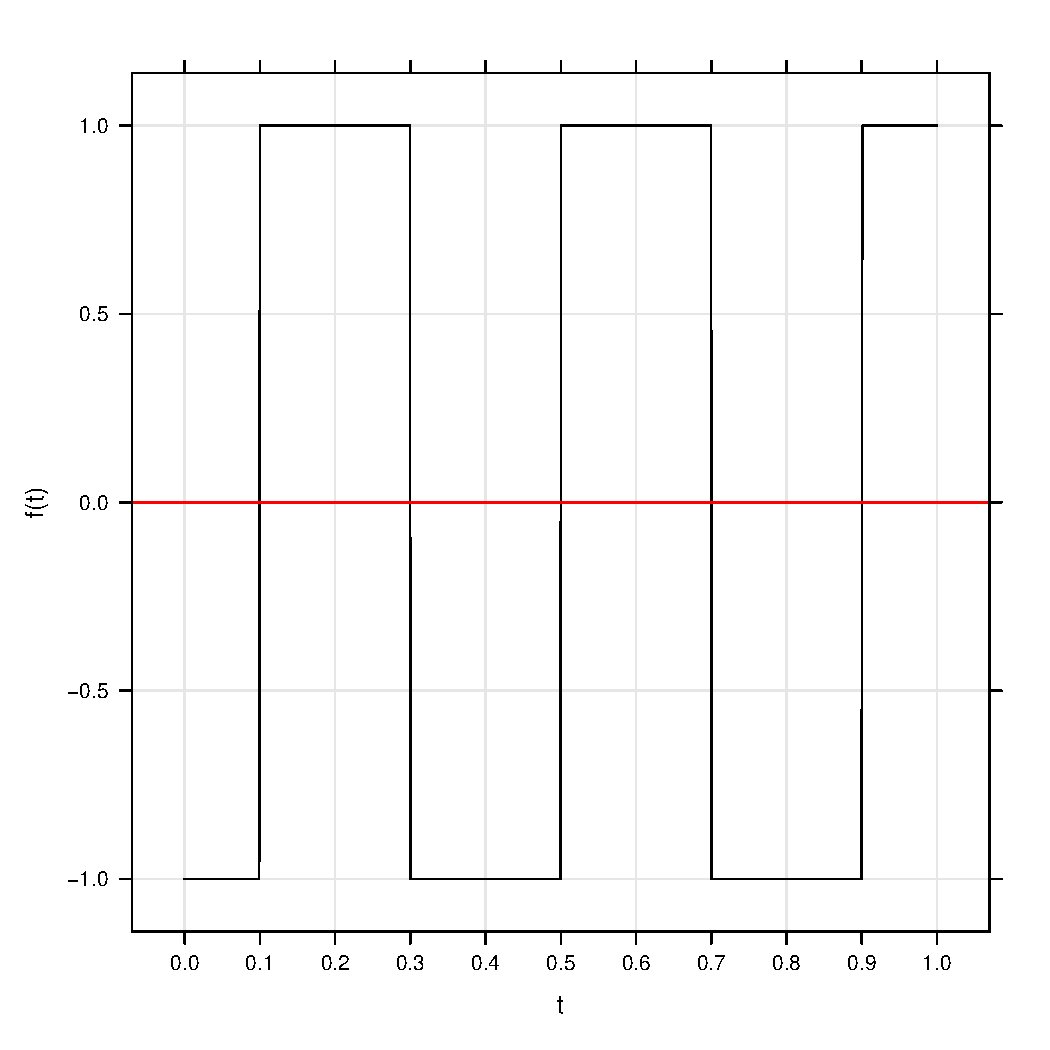
\includegraphics[height=0.52\textheight]{../figs/cuadrada_periodica.pdf}
\end{center}
\end{column}
\end{columns}
\end{frame}

\begin{frame}[label={sec:orgcc0cfa3}]{Clasificación}
\begin{block}{Repetición del valor de la magnitud}
\begin{itemize}
\item Periódicas

El valor de la magnitud se repite de forma regular.

\item No periódicas

El valor de la magnitud varía de forma arbitraria con el tiempo.
\end{itemize}
\end{block}
\begin{columns}
\begin{column}{0.5\columnwidth}
\begin{center}
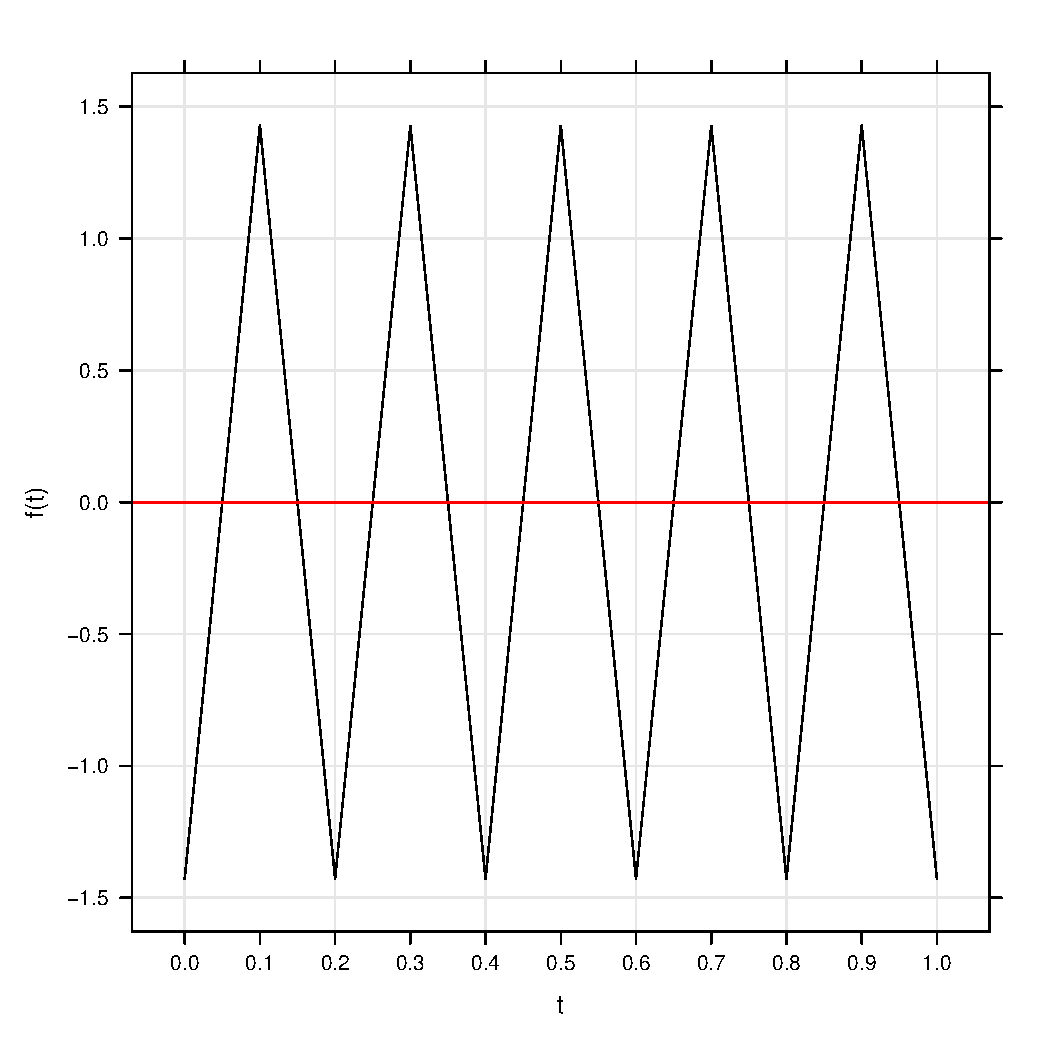
\includegraphics[height=0.52\textheight]{../figs/triangular_periodica.pdf}
\end{center}
\end{column}

\begin{column}{0.5\columnwidth}
\begin{center}
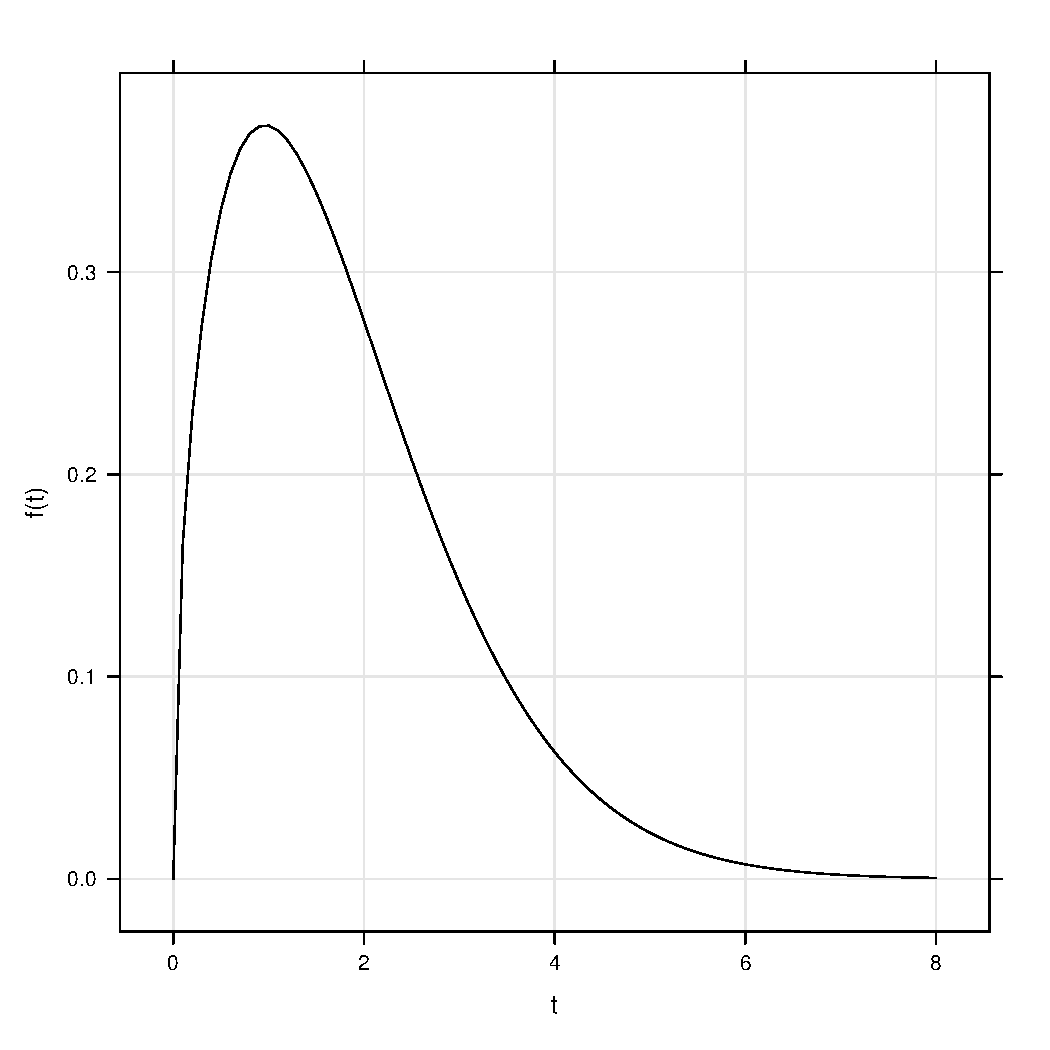
\includegraphics[height=0.52\textheight]{../figs/no_periodica.pdf}
\end{center}
\end{column}
\end{columns}
\end{frame}


\begin{frame}[label={sec:org2103c5f}]{Valores que definen una onda periódica}
\begin{block}{Período y frecuencia}
\begin{itemize}
\item Período (\(T\)): tiempo que tarda en repetirse la función.
\item Frecuencia (\(f\)): número de repeticiones por unidad de tiempo.
\item \(f = \dfrac{1}{T}\)
\end{itemize}
\end{block}
\begin{center}
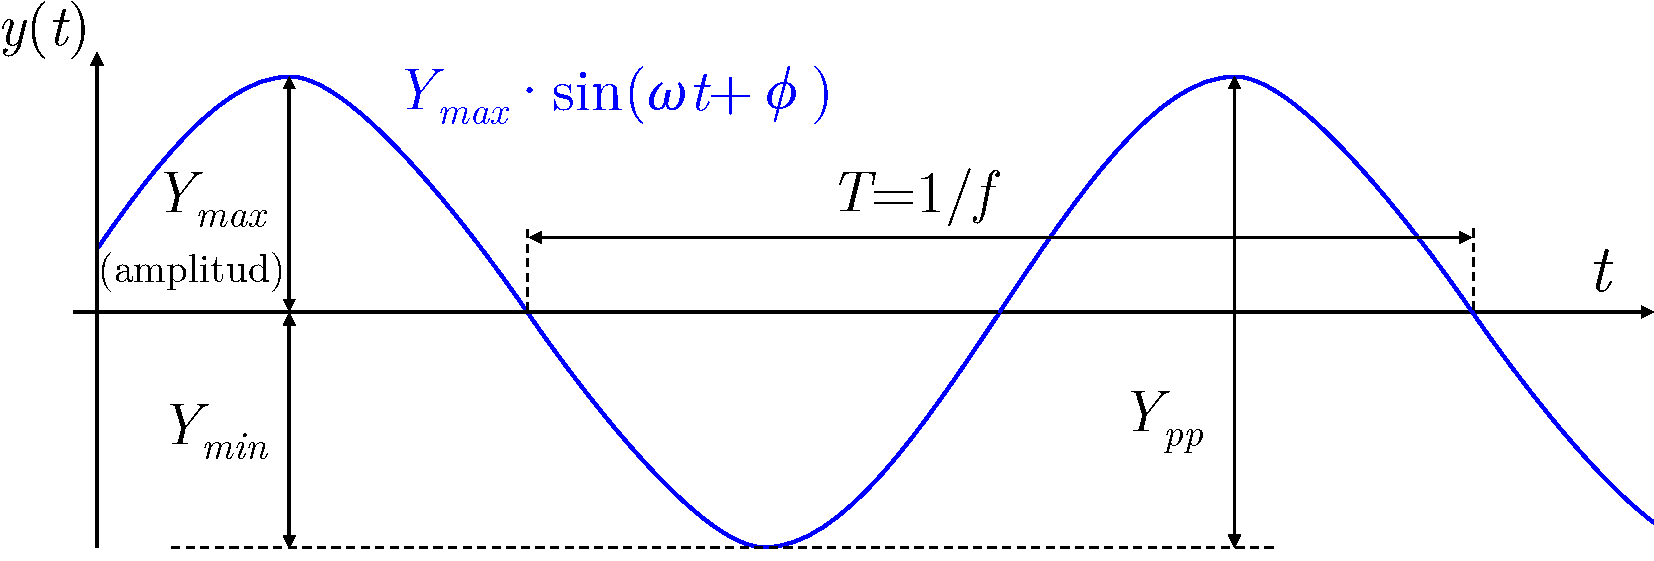
\includegraphics[width=.9\linewidth]{../figs/Senoidal_parametros.pdf}
\end{center}
\end{frame}

\begin{frame}[label={sec:orgacfbdc4}]{Valores que definen una onda periódica}
\begin{itemize}
\item Valores de pico: \(Y_{max} = \max(y(t)) \qquad Y_{min} = \min(y(t))\)

\item Valor pico a pico: \(Y_{pp} = |Y_{max} - Y_{min}|\)
\end{itemize}

\begin{center}
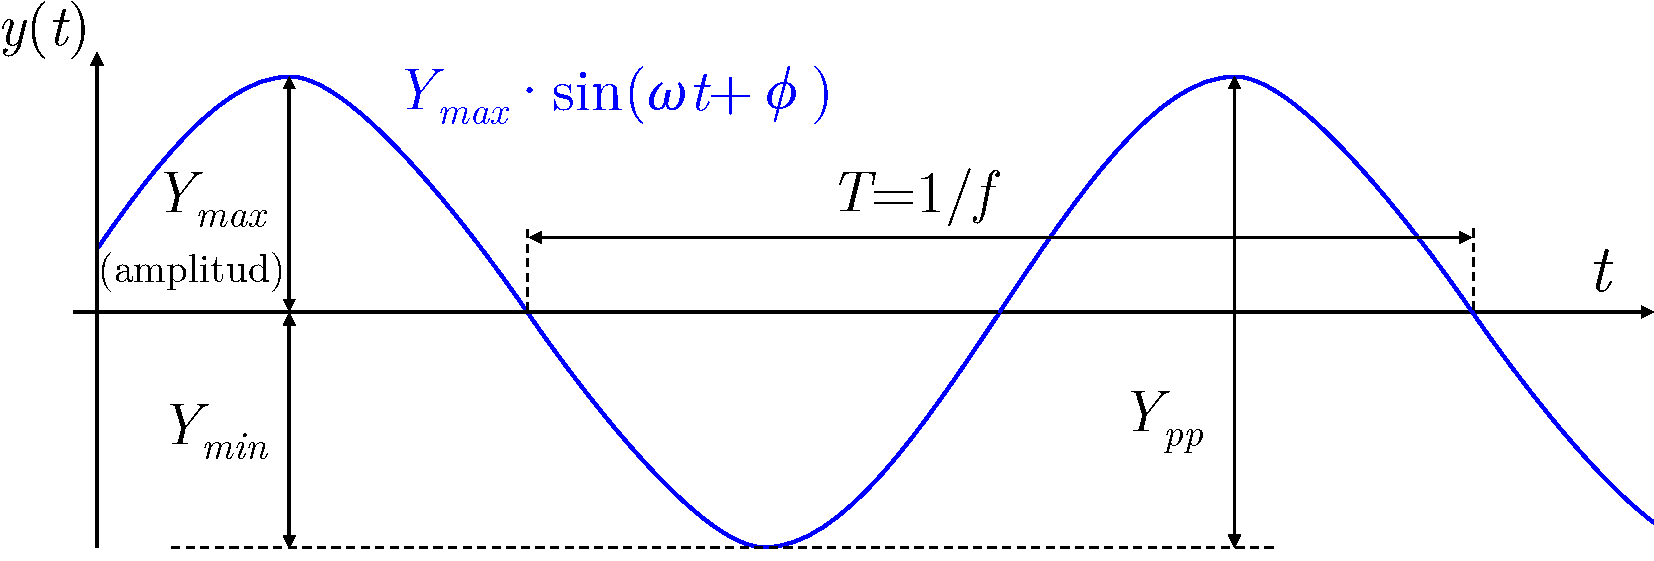
\includegraphics[width=.9\linewidth]{../figs/Senoidal_parametros.pdf}
\end{center}
\end{frame}


\begin{frame}[label={sec:orgb9c4847}]{Valores que definen una onda periódica}
\begin{block}{Valor medio}
\[
U_m=\dfrac{1}{T}\int_T u(t)\, dt \qquad \qquad%
I_m=\dfrac{1}{T}\int_T i(t)\, dt
\]
\end{block}

\begin{block}{Valor eficaz}
\[
U = \sqrt{\dfrac{1}{T}\cdot\int_{T} u^{2}(t)\, dt} \qquad \qquad%
I = \sqrt{\dfrac{1}{T}\cdot\int_{T} i^{2}(t)\, dt}
\]
\end{block}
\end{frame}


\begin{frame}[label={sec:orgb009596}]{Formas de Onda Periódicas}
\framesubtitle{Tren de Pulsos Bidireccional}
\begin{center}
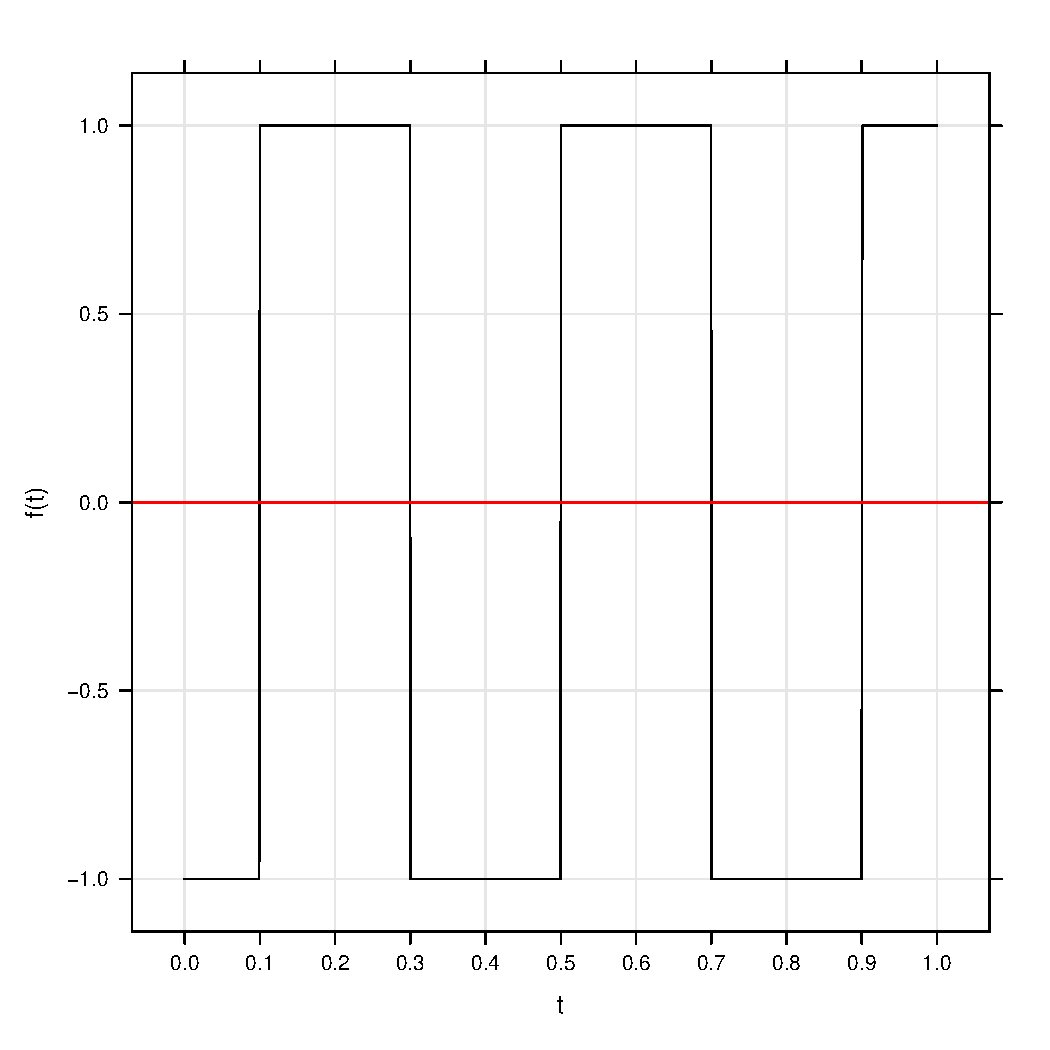
\includegraphics[height=0.9\textheight]{../figs/cuadrada_periodica.pdf}
\end{center}
\end{frame}

\begin{frame}[label={sec:org1498875}]{Formas de Onda Periódicas}
\framesubtitle{Tren de Pulsos Unidireccional}
\begin{center}
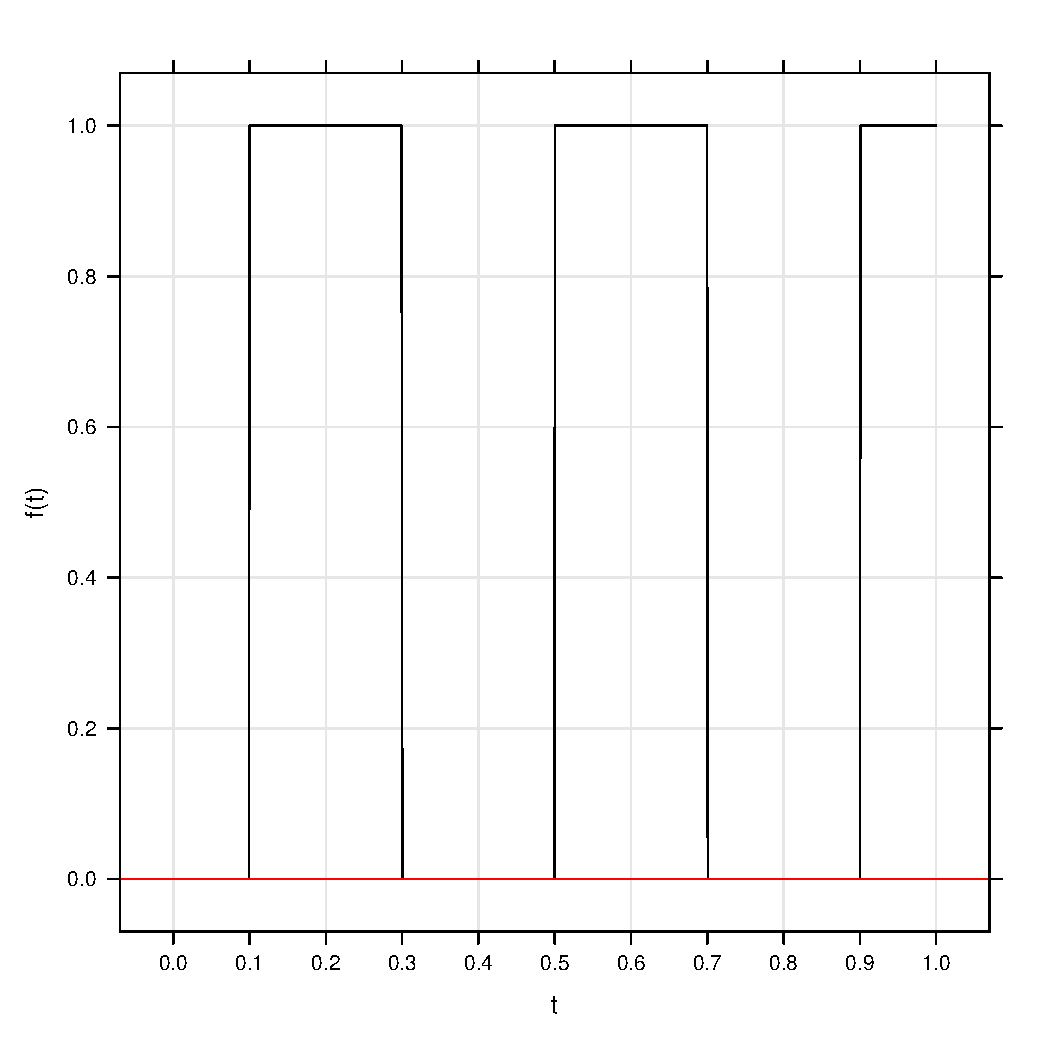
\includegraphics[height=0.9\textheight]{../figs/cuadrada0_periodica.pdf}
\end{center}
\end{frame}

\begin{frame}[label={sec:org5711516}]{Formas de Onda Periódicas}
\framesubtitle{Onda Triangular Bidireccional}
\begin{center}
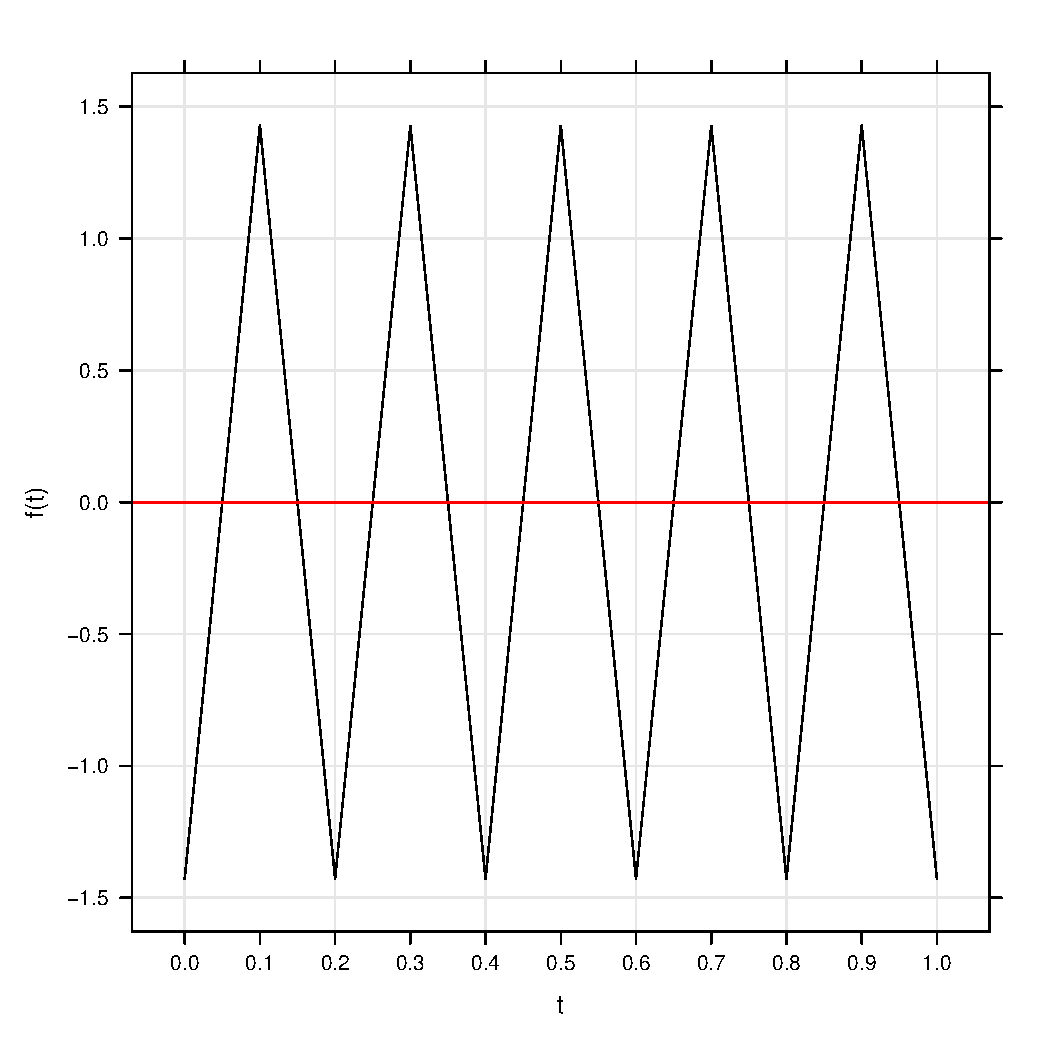
\includegraphics[height=0.9\textheight]{../figs/triangular_periodica.pdf}
\end{center}
\end{frame}
\begin{frame}[label={sec:org5e693d9}]{Formas de Onda Periódicas}
\framesubtitle{Onda Triangular Unidireccional}
\begin{center}
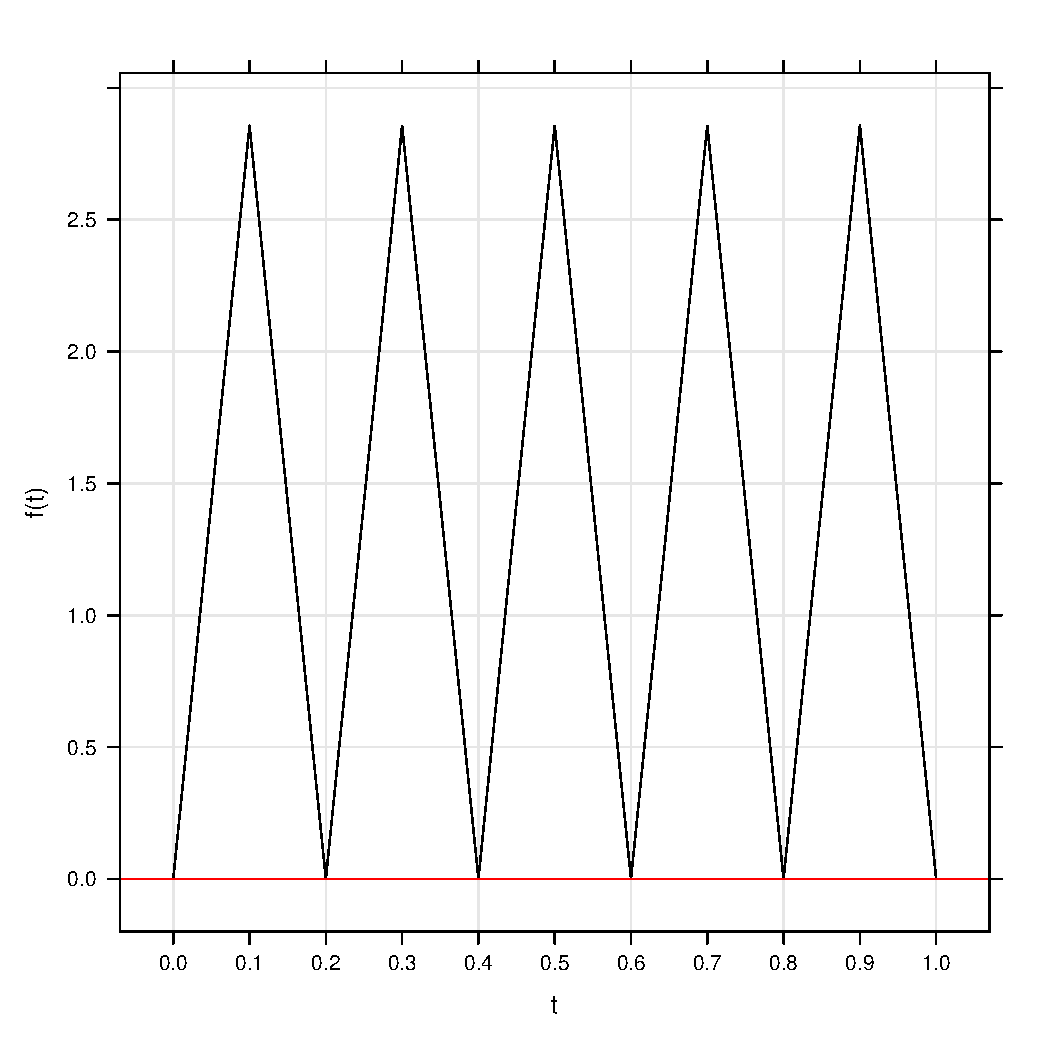
\includegraphics[height=0.9\textheight]{../figs/triangular0_periodica.pdf}
\end{center}
\end{frame}

\begin{frame}[label={sec:orgd0c4d6d}]{Formas de Onda Periódicas}
\framesubtitle{Onda sinusoidal}

\begin{center}
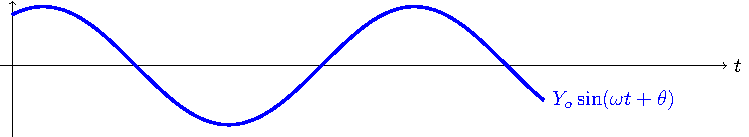
\includegraphics[width=.9\linewidth]{../figs/sin.pdf}
\end{center}
\end{frame}

\section{Onda Sinusoidal}
\label{sec:orgc705ca2}

\begin{frame}[label={sec:org7ec18c3}]{Definición}
\begin{center}
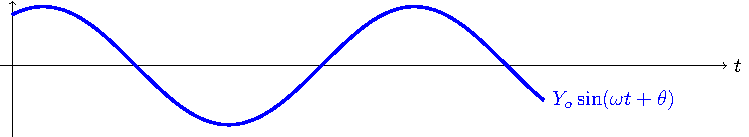
\includegraphics[width=.9\linewidth]{../figs/sin.pdf}
\end{center}


\[
y(t)=Y_{max}\cdot\sen(\omega\cdot t+\theta)
\]

\begin{itemize}
\item \(Y_{max}\) valor máximo de la onda.

\item T: periodo de la onda (segundos)

\item \(\omega=\dfrac{2\cdot\pi}{T}\): pulsación (radianes/segundo)

\item \(f=\dfrac{\omega}{2\cdot\pi}=\dfrac{1}{T}\): frecuencia (Hz)

\item \(\theta\): fase (radianes o grados)
\end{itemize}
\end{frame}


\begin{frame}[label={sec:org699e278}]{Fase}
\begin{center}
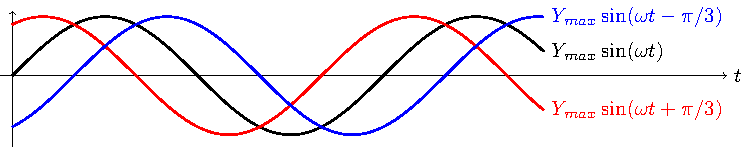
\includegraphics[width=.9\linewidth]{../figs/desfase.pdf}
\end{center}


\[
y(t)=Y_{max}\cdot\sen(\omega\cdot t+\theta)
\]

\begin{itemize}
\item \(\theta\): fase (radianes o grados)

\begin{itemize}
\item Es el argumento de la onda para t=0

\item Tomando una onda como referencia, si la fase es 0º, se dice que
están en fase con la onda de referencia.

\item Si la fase es positiva, se dice que la onda adelanta
respecto a la referencia.
\end{itemize}
\end{itemize}
\end{frame}


\begin{frame}[label={sec:orgdb2dbcd}]{Señales en Cuadratura}
\begin{center}
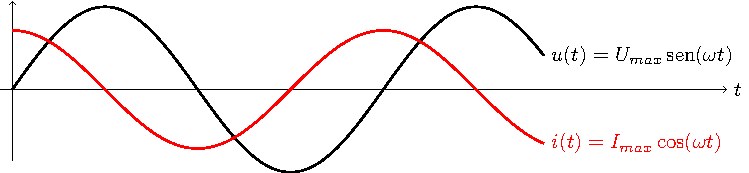
\includegraphics[width=.9\linewidth]{../figs/cuadratura.pdf}
\end{center}

\begin{itemize}
\item Cuando el desfase entre dos señales es de 90º (\(\theta_I - \theta_U = \pi/2\)), se dice que están en cuadratura.
\item El paso por cero de una señal coincide con el paso por el máximo/mínimo de la otra señal.
\end{itemize}
\end{frame}


\begin{frame}[label={sec:org194d81b}]{Valor medio y valor eficaz}
\begin{block}{Valor medio}
\[
Y_m=\dfrac{1}{T}\int_{T} y(t)\, dt
\]

\[
Y_m=\dfrac{1}{T}\int_T Y_{max}\cdot\sen(\omega \cdot t+\theta)\, dt=0
\]
\end{block}
\begin{block}{Valor eficaz}
\[
Y = \sqrt{\dfrac{1}{T}\cdot\int_T y^{2}(t)\, dt}
\]

\[
Y=\sqrt{\dfrac{1}{T}\cdot\int_T \left(Y_{max}\cdot\sen(\omega\cdot t+\theta)\right)^{2}dt}=\boxed{\dfrac{Y_{max}}{\sqrt{2}}}
\]
\end{block}
\end{frame}

\section{Cálculo Fasorial}
\label{sec:orge4ada5f}

\begin{frame}[label={sec:org6268dc0}]{Representación fasorial}
\begin{itemize}
\item Un fasor es un \alert{número complejo} que representa una señal sinusoidal para simplificar cálculos.
\item El \alert{módulo} del fasor es el \alert{valor eficaz}. El \alert{argumento} es la \alert{fase}.
\item Descartamos pulsación: \alert{no} se puede emplear cuando hay frecuencias diferentes en un mismo circuito.
\end{itemize}

\begin{columns}
\begin{column}{0.5\columnwidth}
\begin{align*}
\text{Euler}: \quad \overline{Y} &= Y\cdot e^{j\varphi}\\
\text{Polar}: \quad \overline{Y} &= Y\phase{\varphi}\\
\text{Binómica}: \quad \overline{Y} &= Y\cdot(\cos(\varphi)+\mathrm{j}\cdot\sen(\varphi))
\end{align*}
\end{column}

\begin{column}{0.5\columnwidth}
\begin{center}
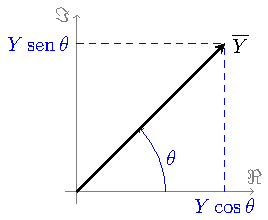
\includegraphics[height=0.55\textheight]{../figs/fasor.pdf}
\end{center}
\end{column}
\end{columns}
\end{frame}

\begin{frame}[label={sec:org2a46e4f}]{Operaciones con fasores}
\begin{align*}
    \overline{Y}_1 & \; = \;         \overbrace{Y_{1}\,\cos(\varphi_1)}^{a_1}+\,\mathrm{j}\,\overbrace{Y_{1}\;\sen(\varphi_1)}^{b_1} 
    \; = \; 
    Y_{1}\phase{\varphi_1}\\
    \overline{Y}_2 & \; = \; \underbrace{Y_{2}\,\cos(\varphi_2)}_{a_2}+\;\mathrm{j}\,\underbrace{Y_{2}\,\sen(\varphi_2)}_{b_2}
    \; = \; 
    Y_2\phase{\varphi_2}
\end{align*}

\begin{block}{Forma binómica:}
\begin{itemize}
\item Suma: \(\quad \overline{Y}_1+\overline{Y}_2 = (a_1+a_2)+\mathrm{j}\,(b_1+b_2)\)
\item Resta: \(\quad \overline{Y}_1-\overline{Y}_2 = (a_1-a_2)+\mathrm{j}\,(b_1-b_2)\)
\end{itemize}
\end{block}
\begin{block}{Forma polar:}
\begin{itemize}
\item Multiplicación: \(\quad \overline{Y}_1\cdot \overline{Y}_2 = (Y_1\cdot Y_2)\phase{\varphi_1+\varphi_2}\)
\item División: \(\quad \dfrac{\overline{Y}_1}{\overline{Y}_2} = \dfrac{Y_{1}}{Y_{2}}\phase{\varphi_1-\varphi_2}\)
\end{itemize}
\end{block}
\end{frame}

\begin{frame}[label={sec:orgf5d087b}]{Tensión y corriente en notación fasorial}
\begin{center}
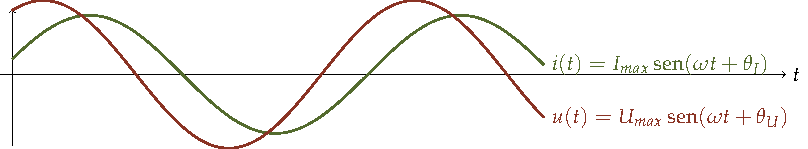
\includegraphics[width=.9\linewidth]{../figs/ondasTensionCorriente.pdf}
\end{center}

\begin{columns}
\begin{column}{0.5\columnwidth}
\begin{align*}
  u(t) = U_{max} \cdot \sen(\omega t + \theta_U) &\rightarrow \overline{U} = U\phase{\theta_U}\\
  i(t) = I_{max} \cdot \sen(\omega t + \theta_I) &\rightarrow \overline{I} = I\phase{\theta_I}
\end{align*}
\end{column}

\begin{column}{0.5\columnwidth}
\begin{center}
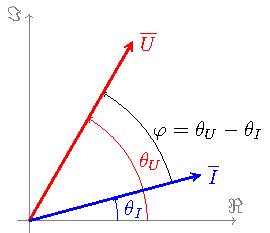
\includegraphics[height=0.5\textheight]{../figs/fasorTensionCorriente.pdf}
\end{center}
\end{column}
\end{columns}
\end{frame}


\begin{frame}[label={sec:org184830b}]{Impedancia: relación entre fasores de tensión y corriente}
\begin{columns}
\begin{column}{0.5\columnwidth}
\begin{align*}
  \overline{U} &= \overline{Z} \cdot \overline{I}\\                 
  \overline{Z} &= \dfrac{\overline{U}}{\overline{I}}
\end{align*}

\[
\boxed{\overline{Z} = \dfrac{U}{I}\phase{\theta_U - \theta_I} \Rightarrow 
    \begin{cases}
      Z = \dfrac{U}{I}\\
      \varphi = \theta_U - \theta_I
    \end{cases}}
\]
\end{column}

\begin{column}{0.5\columnwidth}
\begin{center}
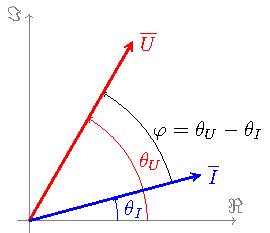
\includegraphics[height=0.5\textheight]{../figs/fasorTensionCorriente.pdf}
\end{center}
\end{column}
\end{columns}
\end{frame}

\begin{frame}[label={sec:orge2b42d4}]{Impedancia Genérica}
\begin{columns}
\begin{column}{0.4\columnwidth}
\begin{align*}
  \overline{Z} &= Z\phase{\varphi}\\[10pt]
	       &= Z \cdot (\cos(\varphi) + j\sen(\varphi))\\[10pt]
	       & = R + j X
\end{align*}
\end{column}

\begin{column}{0.6\columnwidth}
\begin{center}
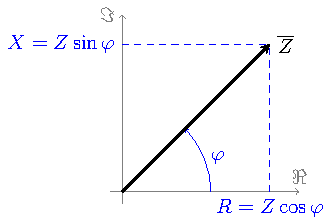
\includegraphics[height=0.6\textheight]{../figs/fasorImpedancia.pdf}
\end{center}
\end{column}
\end{columns}
\end{frame}

\begin{frame}[label={sec:org86ebf38}]{Circuito Resistivo}
Un circuito resistivo no desfasa (\alert{tensión y corriente en fase}).

\begin{center}
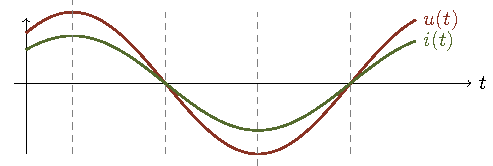
\includegraphics[height=0.4\textheight]{../figs/resistivo.pdf}
\end{center}

\[
    i(t) = I_{max} \cdot \sen(\omega t + \theta_I)
\]
\[
  \begin{rcases}
  u(t) &= {\color{blue}U_{max}} \cdot \sen(\omega t + {\color{red!80} \theta_U}) = \\
  &= R \cdot i(t)=\\
  &= {\color{blue}R \cdot I_{max}} \cdot \sen(\omega t + {\color{red!80}\theta_I + 0})
  \end{rcases} \rightarrow
\begin{cases}
  {\color{blue}U_{max}} &= {\color{blue}R \cdot I_{max}}\\
  {\color{red!80}\theta_U} &= {\color{red!80}\theta_I}
\end{cases}
\]
\end{frame}

\begin{frame}[label={sec:org9bccfff}]{Circuito Resistivo}
Un circuito resistivo no desfasa (\alert{tensión y corriente en fase}).
\begin{center}
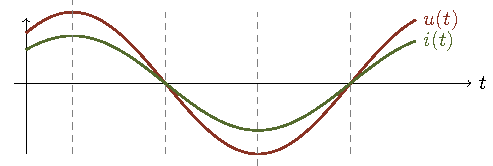
\includegraphics[height=0.3\textheight]{../figs/resistivo.pdf}
\end{center}

\begin{columns}
\begin{column}{0.3\columnwidth}
\begin{align*}
  Z &= \dfrac{U}{I} = R\\
  \varphi &= \theta_U - \theta_I = 0\\
  \Aboxed{\overline{Z}_R &= R \phase{0}}
\end{align*}
\end{column}

\begin{column}{0.35\columnwidth}
\begin{center}
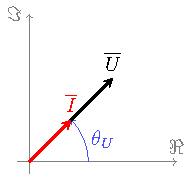
\includegraphics[height=0.35\textheight]{../figs/fasorResistencia_VI.pdf}
\end{center}
\end{column}


\begin{column}{0.35\columnwidth}
\begin{center}
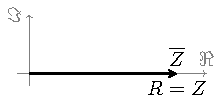
\includegraphics[height=0.25\textheight]{../figs/fasorResistencia.pdf}
\end{center}
\end{column}
\end{columns}
\end{frame}



\begin{frame}[label={sec:org27d21eb}]{Circuito Inductivo puro}
Un circuito inductivo puro genera \alert{señales en cuadratura} y \alert{retrasa la corriente}.
\begin{center}
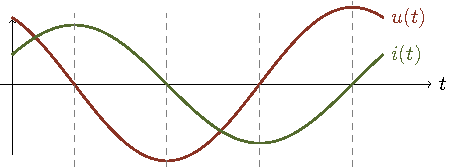
\includegraphics[height=0.4\textheight]{../figs/inductivoPuro.pdf}
\end{center}

\[
    i(t) = I_{max} \cdot \sen(\omega t + \theta_I)
\]
\[
  \begin{rcases}
    u(t) &= {\color{blue}{U_{max}}} \cdot \sen(\omega t +  {\color{red!80}{\theta_U}}) = \\
    &= L \cdot \dfrac{d i(t)}{dt} =\\
    &= {\color{blue}{\omega L \cdot I_{max}}} \cdot \sen(\omega t + {\color{red!80}{\theta_I +\pi/2}})
  \end{rcases} \rightarrow
\begin{cases}
  {\color{blue}U_{max}} &= {\color{blue}\omega L \cdot I_{max}}\\
  {\color{red!80}\theta_U} &= {\color{red!80}\theta_I + \pi/2}
\end{cases}
\]
\end{frame}


\begin{frame}[label={sec:orga6e1def}]{Circuito Inductivo puro}
Un circuito inductivo puro genera \alert{señales en cuadratura} y \alert{retrasa la corriente}.

\begin{center}
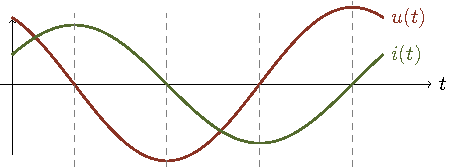
\includegraphics[height=0.3\textheight]{../figs/inductivoPuro.pdf}
\end{center}

\begin{columns}
\begin{column}{0.3\columnwidth}
\begin{align*}
  Z &= \dfrac{U}{I} = \omega L\\
  \varphi &= \theta_U - \theta_I = \pi/2\\
  \Aboxed{\overline{Z}_L &= j\omega L = \omega L \phase{\ang{90}}}
\end{align*}
\end{column}


\begin{column}{0.4\columnwidth}
\begin{center}
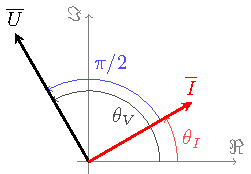
\includegraphics[height=0.4\textheight]{../figs/fasorInductancia_VI.pdf}
\end{center}
\end{column}


\begin{column}{0.3\columnwidth}
\begin{center}
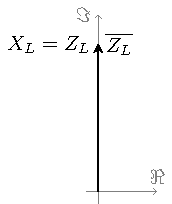
\includegraphics[height=0.4\textheight]{../figs/fasorInductancia.pdf}
\end{center}
\end{column}
\end{columns}
\end{frame}


\begin{frame}[label={sec:orgce83eb0}]{Circuito Capacitivo puro}
Un circuito capacitivo puro genera \alert{señales en cuadratura} y \alert{adelanta la corriente}.

\begin{center}
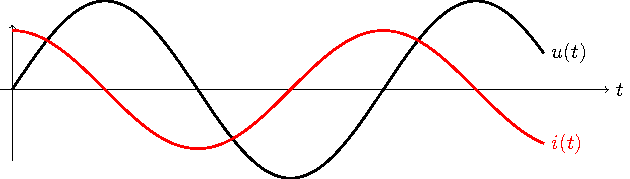
\includegraphics[height=0.4\textheight]{../figs/capacitivoPuro.pdf}
\end{center}

\[
    i(t) = I_{max} \cdot \sen(\omega t + \theta_I)
\]
\[
\begin{rcases}
  u(t) &= {\color{blue}{U_{max}}} \cdot \sen(\omega t + {\color{red!80}{\theta_U}}) = \\
  &= 1/C \cdot \int_{-\infty}^ t i(\tau)d\tau =\\
  &= {\color{blue}{\dfrac{1}{\omega C} \cdot I_{max}}} \cdot \sen(\omega t + {\color{red!80}{\theta_I -\pi/2}})
\end{rcases} \rightarrow
\begin{cases}
  {\color{blue}U_{max}} &= {\color{blue}\dfrac{1}{\omega C} \cdot I_{max}}\\
  {\color{red!80}\theta_U} &= {\color{red!80}\theta_I - \pi/2}
\end{cases}
\]
\end{frame}


\begin{frame}[label={sec:orgf120d7a}]{Circuito Capacitivo puro}
Un circuito capacitivo puro genera \alert{señales en cuadratura} y \alert{adelanta la corriente}.

\begin{center}
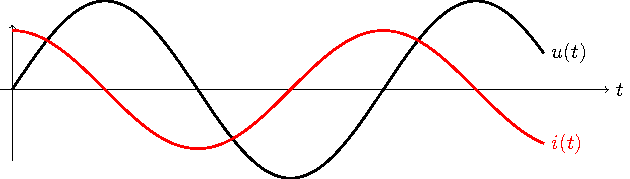
\includegraphics[height=0.3\textheight]{../figs/capacitivoPuro.pdf}
\end{center}

\begin{columns}
\begin{column}{0.3\columnwidth}
\begin{align*}
  Z &= \dfrac{U}{I} = \dfrac{1}{\omega C}\\
  \varphi &= \theta_U - \theta_I = - \pi/2\\
  \Aboxed{\overline{Z}_C &= \dfrac{1}{j\omega C} = \dfrac{1}{\omega C}\phase{\ang{-90}}}
\end{align*}
\end{column}


\begin{column}{0.4\columnwidth}
\begin{center}
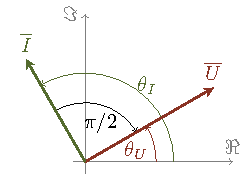
\includegraphics[height=0.4\textheight]{../figs/fasorCondensador_VI.pdf}
\end{center}
\end{column}


\begin{column}{0.3\columnwidth}
\begin{center}
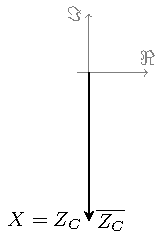
\includegraphics[height=0.4\textheight]{../figs/fasorCondensador.pdf}
\end{center}
\end{column}
\end{columns}
\end{frame}

\begin{frame}[label={sec:org1936291}]{Resumen}
\begin{columns}
\begin{column}{0.6\columnwidth}
\[
  \begin{array}{lccc}
    \text{Elemento} & \text{Impedancia} & \text{Módulo} & \text{Ángulo}\\
    \hline\\
    \text{\color{darkolivegreen}Resistencia} & \color{darkolivegreen}R & \color{darkolivegreen}R & \color{darkolivegreen}0\\
    \text{\color{frenchblue}Bobina} & \color{frenchblue}j \omega L & \color{frenchblue} \omega L & \color{frenchblue} \ang{90}\\
     \text{\color{burgundy}Condensador} & \color{burgundy} 1/(j \omega C) & \color{burgundy} 1/(\omega C) & \color{burgundy} \ang{-90}\\
  \end{array}
\]
\end{column}

\begin{column}{0.5\columnwidth}
\begin{center}
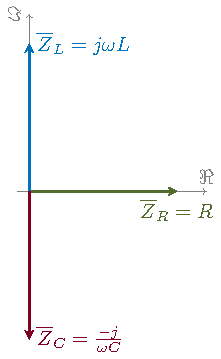
\includegraphics[height=0.8\textheight]{../figs/ResumenImpedancias.pdf}
\end{center}
\end{column}
\end{columns}
\end{frame}

\begin{frame}[label={sec:org2fdfb7c}]{Circuito RL (inductivo con pérdidas)}
\begin{center}
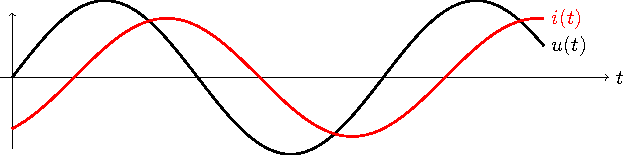
\includegraphics[height=0.25\textheight]{../figs/inductivo.pdf}
\end{center}
\begin{columns}
\begin{column}{0.45\columnwidth}
\begin{center}
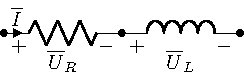
\includegraphics[width=0.8\textwidth]{../figs/RL.pdf}
\end{center}
\end{column}


\begin{column}{0.55\columnwidth}
\begin{center}
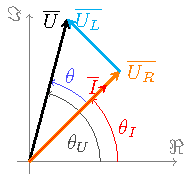
\includegraphics[height=0.5\textheight]{../figs/fasorInductanciaReal_VI.pdf}
\end{center}
\end{column}
\end{columns}
\end{frame}

\begin{frame}[label={sec:org352744c}]{Circuito RL (inductivo con pérdidas)}
\begin{center}
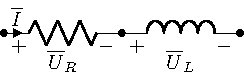
\includegraphics[height=0.2\textheight]{../figs/RL.pdf}
\end{center}

\[
\begin{rcases}
  \overline{U}_R &= R \overline{I}\\
  \overline{U}_L &= j\omega L \overline{I}
\end{rcases} \rightarrow \quad
    \begin{aligned}
      \overline{U} &= \overline{U}_R + \overline{U}_L =\\
		   &=(R + j\omega L) \overline{I}
    \end{aligned}
\]
\end{frame}
\begin{frame}[label={sec:org3dc2894}]{Circuito RL (inductivo con pérdidas)}
\begin{center}
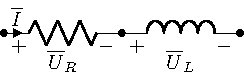
\includegraphics[height=0.2\textheight]{../figs/RL.pdf}
\end{center}

\begin{columns}
\begin{column}{0.45\columnwidth}
\[
\overline{Z} = R + j\omega L \Rightarrow \boxed{\varphi > 0}
\]
\[
  |Z| = \sqrt{R^2 + (\omega L)^2}
\]
\[
  \varphi = \atan{\dfrac{\omega L}{R}}
\]
\end{column}

\begin{column}{0.55\columnwidth}
\begin{center}
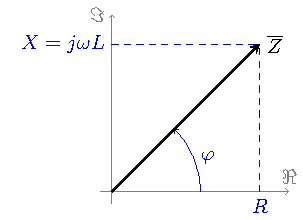
\includegraphics[width=.9\linewidth]{../figs/fasorInductanciaReal.pdf}
\end{center}
\end{column}
\end{columns}
\end{frame}


\begin{frame}[label={sec:org0ad198e}]{Circuito RC (capacitivo con pérdidas)}
\begin{center}
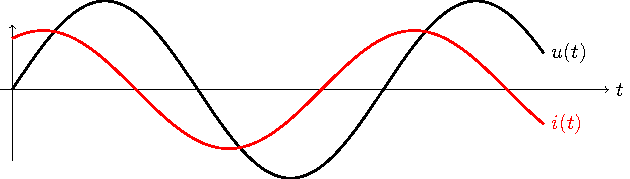
\includegraphics[height=0.25\textheight]{../figs/capacitivo.pdf}
\end{center}


\begin{columns}
\begin{column}{0.45\columnwidth}
\begin{center}
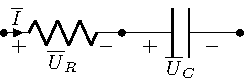
\includegraphics[width=0.8\textwidth]{../figs/RC.pdf}
\end{center}
\end{column}

\begin{column}{0.55\columnwidth}
\begin{center}
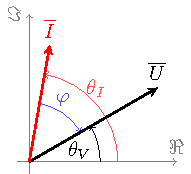
\includegraphics[height=0.45\textheight]{../figs/fasorCondensadorReal_VI.pdf}
\end{center}
\end{column}
\end{columns}
\end{frame}


\begin{frame}[label={sec:orga317e32}]{Circuito RC (capacitivo con pérdidas)}
\begin{center}
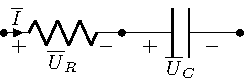
\includegraphics[height=0.2\textheight]{../figs/RC.pdf}
\end{center}

\[
\begin{rcases}
  \overline{U}_R &= R \overline{I}\\
  \overline{U}_C &= -j \dfrac{1}{\omega C} \overline{I}
\end{rcases} \rightarrow \quad
\begin{aligned}
  \overline{U} &= \overline{U}_R + \overline{U}_C =\\
               &= (R - j \dfrac{1}{\omega C}) \overline{I} 
\end{aligned}
\]
\end{frame}
\begin{frame}[label={sec:org00311ca}]{Circuito RC (capacitivo con pérdidas)}
\begin{center}
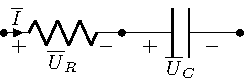
\includegraphics[height=0.2\textheight]{../figs/RC.pdf}
\end{center}

\begin{columns}
\begin{column}{0.45\columnwidth}
\[
\overline{Z} = R - \dfrac{j}{\omega C} \Rightarrow \boxed{\varphi < 0}
\]

\[
  |Z| = \sqrt{R^2 + \dfrac{1}{(\omega C)^2}}
\]

\[
  \varphi = - \atan{\dfrac{1}{\omega R C}}
\]
\end{column}

\begin{column}{0.55\columnwidth}
\begin{center}
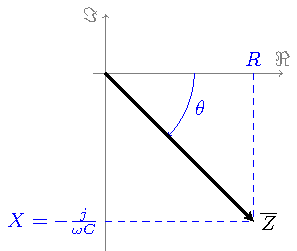
\includegraphics[height=0.45\textheight]{../figs/fasorCondensadorReal.pdf}
\end{center}
\end{column}
\end{columns}
\end{frame}


\begin{frame}[label={sec:orga8cf945}]{Circuito RLC serie}
\begin{center}
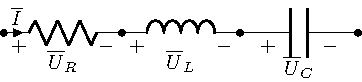
\includegraphics[height=0.2\textheight]{../figs/RLC.pdf}
\end{center}

\[
\begin{rcases}
  \overline{U}_R &= R \overline{I}\\
  \overline{U}_L &= j\omega L \overline{I}\\
  \overline{U}_C &= -j \dfrac{1}{\omega C} \overline{I}
\end{rcases} \rightarrow \quad
\begin{aligned}
  \overline{U} &= \overline{U}_R + \overline{U}_L + \overline{U}_C =\\
               &= \left(R + j(\omega L - \dfrac{1}{\omega C})\right) \overline{I} 
\end{aligned}
\]
\end{frame}

\begin{frame}[label={sec:org64d67c8}]{Circuito RLC serie}
\begin{center}
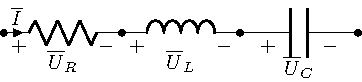
\includegraphics[height=0.2\textheight]{../figs/RLC.pdf}
\end{center}

\begin{columns}
\begin{column}{0.4\columnwidth}
\[
\overline{Z} = R + j(\omega L - \dfrac{1}{\omega C})
\]
\[
  |Z| = \sqrt{R^2 + (\omega L - \dfrac{1}{\omega C})^2}
\]
\[
  \varphi = \atan{\dfrac{\omega L - \dfrac{1}{\omega C}}{R}}
\]
\end{column}

\begin{column}{0.6\columnwidth}
\begin{itemize}
\item \(\varphi > 0 \Rightarrow \omega L > \dfrac{1}{\omega C}\): inductivo
\item \(\varphi < 0 \Rightarrow \omega L < \dfrac{1}{\omega C}\): capacitivo
\item \(\varphi = 0 \Rightarrow \omega L = \dfrac{1}{\omega C}\): resistivo (resonancia)
\end{itemize}
\end{column}
\end{columns}

\[
\boxed{u(t) = Z \cdot I_{max} \sen(\omega t + \theta_I + \varphi)}
\]
\end{frame}

\begin{frame}[label={sec:orgc09ee3a}]{Circuito serie general}
\begin{columns}
\begin{column}{0.6\columnwidth}
\begin{center}
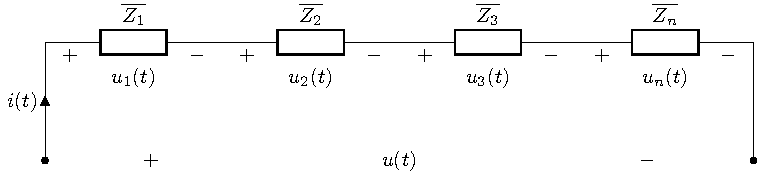
\includegraphics[width=.9\linewidth]{../figs/serie_general.pdf}
\end{center}
\end{column}


\begin{column}{0.1\columnwidth}
\(\LARGE \xrightarrow{\hspace*{0.5cm}}\)
\end{column}

\begin{column}{0.3\columnwidth}
\begin{center}
\includegraphics[width=.9\linewidth]{../figs/serie_general_eq.pdf}
\end{center}
\end{column}
\end{columns}

\[\overline{U} = \overline{U}_1+\overline{U}_2+...+\overline{U}_n \; = \; \overline{I} \cdot(\overline{Z}_1+\overline{Z}_2+...+\overline{Z}_n) \; = \; \overline{I}\cdot\overline{Z}_{eq}\]


\[{\Large \boxed{ \overline{Z}_{eq} = \sum_{i=1}^n \overline{Z}_i} }\]

\[R_{eq}=\sum_{i=1}^n R_i\,\qquad \qquad X_{eq}=\sum_{i=1}^n X_i\]

\[\varphi=\arctan\left(\dfrac{X_{eq}}{R_{eq}}\right)\]
\end{frame}

\begin{frame}[label={sec:orga0dcc78}]{Circuito paralelo general}
\begin{columns}
\begin{column}{0.6\columnwidth}
\begin{center}
\begin{center}
\includegraphics[width=.9\linewidth]{../figs/paralelo_general.pdf}
\end{center}
\end{center}
\end{column}

\begin{column}{0.1\columnwidth}
\begin{center}
\(\LARGE \xrightarrow{\hspace*{0.5cm}}\)
\end{center}
\end{column}

\begin{column}{0.2\columnwidth}
\begin{center}
\begin{center}
\includegraphics[width=.9\linewidth]{../figs/paralelo_general_eq.pdf}
\end{center}
\end{center}
\end{column}
\end{columns}


\[\overline{I} = \overline{I}_1+\overline{I}_2+...+\overline{I}_n \; = \; \overline{U} \cdot\left(\dfrac{1}{\overline{Z}_1}+\dfrac{1}{\overline{Z}_2}+...+\dfrac{1}{\overline{Z}_n}\right) \; = \; \dfrac{\overline{U}}{\overline{Z}_{eq}}\]

\[
  \boxed{\dfrac{1}{\overline{Z}_{eq}}=\sum_{i=1}^n \dfrac{1}{\overline{Z}_i}}%
  \Rightarrow%
  \boxed{\overline{Y}_{eq}=\sum_{i=1}^n \overline{Y}_i}
\]
\end{frame}


\begin{frame}[label={sec:orgb99611e}]{Impedancia y Admitancia}
\[
\boxed{
  \overline{Y} = \dfrac{1}{\overline{Z}} \rightarrow \left\{%
    \begin{array}{l}
    |\overline{Y}| = \dfrac{1}{|\overline{Z}|}\\[12pt]
    \varphi_Y = -\varphi_Z = - \varphi\\
    \end{array}\right.
      }
\]

\begin{columns}
\begin{column}{0.5\columnwidth}
\begin{center}
\includegraphics[height=0.1\textheight]{../figs/Z.pdf}
\end{center}
\[
  \overline{U} = \overline{Z} \cdot \overline{I}
\]
\[
  \overline{Z} = R + j X
\]
\end{column}

\begin{column}{0.5\columnwidth}
\begin{center}
\includegraphics[height=0.25\textheight]{../figs/Y.pdf}
\end{center}
\[
  \overline{I} = \overline{Y} \cdot \overline{U}
\]
\[
  \overline{Y} = G + j B
\]
\end{column}
\end{columns}
\end{frame}

\section{Potencia}
\label{sec:orgf851733}
\begin{frame}[label={sec:org9f9df95}]{Expresión general}
Sea la tensión referencia de fases. Si \(\varphi > 0\) (inductivo) la corriente está retrasada respecto de la tensión (\emph{circuito en retraso}).
\begin{align*}
  u(t) &= U_{max} \cos \omega t\\
  i(t) &= I_{max} \cos (\omega t {\color{red}-} \varphi)\\
  p(t) &= u(t) \cdot i(t)
\end{align*}
\end{frame}
\begin{frame}[label={sec:orgf3dfc6a}]{Expresión general}
\begin{align*}
  p(t) &= (\sqrt{2} \cdot U \cdot \cos(\omega t)) \cdot (\sqrt{2} \cdot I \cdot \cos(\omega t - \varphi)) =\\
       &= 2 \cdot U \cdot I \cdot \cos(\omega t)\cdot \cos(\omega t - \varphi) =\\
       &= U I \cdot \left( \cos(2\omega t - \varphi) + \cos(\varphi)\right) =\\
       &= U I \cdot \left(\cos(2\omega t)\cos(\varphi) + \sen(2\omega t)\sen(\varphi) +  \cos(\varphi)\right)
\end{align*}

\begin{equation*}
  \boxed{p(t) = U I \cos(\varphi) + U I \cos(\varphi) \cos(2\omega t) + U I \sen(\varphi) \sen(2\omega t)}
\end{equation*}
\end{frame}
\begin{frame}[label={sec:orgf460ae9}]{Expresión general}
\begin{equation*}
  p(t) = {\color{blue}U I \cos(\varphi)} + {\color{blue}U I \cos(\varphi)} \cos(2\omega t) + {\color{red}U I \sen(\varphi)} \sen(2\omega t)
\end{equation*}

\[
  \color{blue}P = UI\cos\varphi \quad%
  \color{red}Q = UI\sen\varphi
\]

\begin{equation*}
  \boxed{p(t) = {\color{blue}P} \cdot (1 + \cos(2\omega t)) + {\color{red}Q} \cdot \sen(2\omega t)}
\end{equation*}
\end{frame}


\begin{frame}[label={sec:org9178778}]{Circuito Resistivo}
   \[
     P = UI\cos\varphi \quad%
     {\color{gray}Q = UI\sen\varphi}
   \]
   
   \begin{equation*}
p(t) = P \cdot (1 + \cos(2\omega t)) + {\color{gray}Q \cdot \sen(2\omega t)}
\end{equation*}

\noindent\rule{\textwidth}{0.5pt}
\[
  \varphi = 0 \rightarrow%
  \left\{% 
    \begin{array}{l}
      P = UI = U^2/R = I^2 R\\
      Q = 0\\
    \end{array}
    \right.
  \]

  \[
    p(t) = P \cdot (1 + \cos(2 \omega t))
  \]
\end{frame}

\begin{frame}[label={sec:org1645283}]{Circuito Resistivo}
\begin{center}
\includegraphics[width=.9\linewidth]{../figs/resistivoPotencia.pdf}
\end{center}

\begin{itemize}
\item Fluctúa al doble de frecuencia.
\item Es siempre positiva.
\end{itemize}
\end{frame}

\begin{frame}[label={sec:orgb0cdc3c}]{Circuito Inductivo puro}
   \[
     {\color{gray}P = UI\cos\varphi} \quad%
     Q = UI\sen\varphi
   \]
   
   \begin{equation*}
p(t) = {\color{gray}P \cdot (1 + \cos(2\omega t))} + Q \cdot \sen(2\omega t)
\end{equation*}

\noindent\rule{\textwidth}{0.5pt}

\[
  \varphi = \pi/2 \rightarrow%
  \left\{% 
    \begin{array}{l}
      P = 0\\
      Q = UI = \dfrac{U^2}{\omega L} = I^2 \omega L\\
    \end{array}
    \right.
  \]

\[
  p(t) = Q \cdot \sen(2 \omega t)
\]
\end{frame}

\begin{frame}[label={sec:org5aeadd0}]{Circuito Inductivo puro}
\begin{center}
\includegraphics[width=.9\linewidth]{../figs/inductivoPuroPotencia.pdf}
\end{center}

\begin{itemize}
\item Fluctúa al doble de frecuencia.
\item Pasa por los ceros de tensión y corriente.
\item Su valor medio es nulo.
\end{itemize}
\end{frame}

\begin{frame}[label={sec:org7ef37be}]{Circuito Capacitivo puro}
   \[
     {\color{gray}P = UI\cos\varphi} \quad%
     Q = UI\sen\varphi
   \]
   
   \begin{equation*}
p(t) = {\color{gray}P \cdot (1 + \cos(2\omega t))} + Q \cdot \sen(2\omega t)
\end{equation*}

\noindent\rule{\textwidth}{0.5pt}

\[
  \varphi = -\pi/2 \rightarrow%
  \left\{% 
    \begin{array}{l}
      P = 0\\
      Q = -UI = -U^2 \omega C = - \dfrac{I^2}{\omega C}\\
    \end{array}
    \right.
  \]
\[
  p(t) = Q \cdot \sen(2 \omega t)
\]
\end{frame}

\begin{frame}[label={sec:org85a516e}]{Circuito Capacitivo puro}
\begin{center}
\includegraphics[width=.9\linewidth]{../figs/capacitivoPuroPotencia.pdf}
\end{center}

\begin{itemize}
\item Fluctúa al doble de frecuencia.
\item Pasa por los ceros de tensión y corriente.
\item Su valor medio es nulo.
\end{itemize}
\end{frame}

\begin{frame}[label={sec:orgec3f726}]{Circuito Inductivo con pérdidas}
\begin{center}
\includegraphics[height=0.5\textheight]{../figs/inductivoPotencia.pdf}
\end{center}

\[
     p(t) = P \cdot (1 + \cos(2\omega t)) + Q \cdot \sen(2\omega t)
\]

\begin{center}
Valor medio positivo, \(P = U I \cos \varphi\)
\end{center}
\end{frame}


\begin{frame}[label={sec:orgfdd975b}]{Circuito Capacitivo con pérdidas}
\begin{center}
\includegraphics[height=0.5\textheight]{../figs/capacitivoPotencia.pdf}
\end{center}

\[
     p(t) = P \cdot (1 + \cos(2\omega t)) + Q \cdot \sen(2\omega t)
\]

\begin{center}
Valor medio positivo, \(P = U I \cos \varphi\)
\end{center}
\end{frame}

\begin{frame}[label={sec:org0c8e3ef}]{Triángulo de Potencias}
\begin{columns}
\begin{column}{0.4\columnwidth}
\begin{itemize}
\item Potencia Activa [\(W\)]
\end{itemize}
\[  
\boxed{P = U\cdot I\cdot\cos(\varphi) = R \cdot I^2}
\]

\begin{itemize}
\item Potencia Reactiva [\(var\)]
\end{itemize}
\[
\boxed{Q = U\cdot I\cdot\sen(\varphi) = X \cdot I^2}
\]

\begin{itemize}
\item Potencia Aparente [\(VA\)]
\end{itemize}
\[
\boxed{\overline{S} = P + jQ = \overline{U} \cdot \overline{I}^*}
\]

{\footnotesize\begin{align*}
  \overline{U} &= U\phase{0}\\
  \overline{I} &= I\phase{-\varphi}\\
                \overline{U} \overline{I}^* &= U\phase{0} \cdot I\phase{\varphi} = UI\phase{\varphi}\\
                &= U I (\cos\varphi + j \sen\varphi) = \\
                &= P + j Q
\end{align*}}
\end{column}

\begin{column}{0.6\columnwidth}
\begin{center}
\includegraphics[width=.9\linewidth]{../figs/trianguloPotencias.pdf}
\end{center}

\[
|S| = U \cdot I
\]
\[
\varphi_S = \varphi_Z = \varphi
\]
\[
f.d.p. \equiv \cos(\varphi)
\]
\end{column}
\end{columns}
\end{frame}
\begin{frame}[label={sec:orga3736dd}]{Potencia de elementos}
\begin{center}
\begin{tabular}{lccccl}
\toprule
\large \alert{Elemento} & \large \alert{\(\varphi\)} & \large \alert{\(P\)} & \large \alert{\(Q\)} & \large \alert{\(\overline{S}\)} & \large \alert{Comentarios}\\
\midrule
Resistencia & 0 & \(R I^2\) & 0 & \((R I^2) \phase{0}\) & - Consume potencia activa\\
 &  &  &  &  & - No consume potencia reactiva\\
\midrule
Inductancia & \(\pi\)/2 & 0 & \(\omega L I^2\) & \((\omega L I^2) \phase{\pi/2}\) & - No consume potencia activa\\
 &  &  &  &  & - Consume potencia reactiva\\
\midrule
Condensador & -\(\pi\)/2 & 0 & \(- \omega C U^2\) & \(\omega C U^2 \phase{-\pi/2}\) & - No consume potencia activa\\
 &  &  &  &  & - Genera potencia reactiva\\
\bottomrule
\end{tabular}
\end{center}
\end{frame}


\begin{frame}[label={sec:org67884d7}]{Teorema de Boucherot}
\begin{itemize}
\item En un circuito con múltiples elementos, la potencia aparente total es la suma de las potencias aparentes individuales.
\end{itemize}
\begin{align*}
  \overline{S} &= \sum_{i = 1}^{n} \overline{S}_i\\
  P + jQ &= \sum^n_{i = 1} (P_i + jQ_i)
\end{align*}

\begin{itemize}
\item La potencia activa (reactiva) total es la suma de las potencias activas (reactivas) individuales.
\end{itemize}

\begin{align*}
P &= \sum_{i = 1}^n P_i\\
Q &= \sum_{i = 1}^n Q_i
\end{align*}
\end{frame}

\begin{frame}[label={sec:orgdd35afc}]{Medida de potencia}
\begin{center}
\includegraphics[height=0.7\textheight]{../figs/vatimetro.pdf}
\end{center}

\alert{Vatímetro}: equipo de medida de 4 terminales (1 par para tensión, 1 par para corriente)
\end{frame}

\begin{frame}[label={sec:orgd6427b5}]{Medida de potencia}
\begin{center}
\includegraphics[height=0.5\textheight]{../figs/vatimetro_Z.pdf}
\end{center}


Habitualmente se emplea con 3 terminales cortocircuitando terminales con *.
\[
  \boxed{W = |V| |I| \cos(\varphi_V - \varphi_I) = P_Z}
\]
\end{frame}

\section{Compensación de reactiva}
\label{sec:org1785e1e}

\begin{frame}[label={sec:org154e7a0}]{Factor de potencia}
El factor de potencia, \(\cos(\varphi)\), representa la aportación de potencia activa dentro de la potencia aparente.
\[
P = S \cos \varphi
\]

Sean dos sistemas con \alert{misma tensión y potencia activa}, y factores de potencia \(\cos \varphi_2 < \cos \varphi_1\) (\(Q_2 > Q_1\))

\begin{center}
\includegraphics[height=0.5\textheight]{../figs/Fasores_CompensacionReactiva.pdf}
\end{center}
\end{frame}

\begin{frame}[label={sec:org2297188}]{Potencia Aparente}
\begin{center}
\includegraphics[height=0.5\textheight]{../figs/Fasores_CompensacionReactiva.pdf}
\end{center}


El sistema 2 requiere \alert{mayor potencia aparente} (generador mayor) para alimentar la misma potencia activa.
\[
  \left(\dfrac{P}{\cos \varphi_1} = S_1 \right) < \left( S_2 = \dfrac{P}{\cos \varphi_2}\right) 
\]
\end{frame}

\begin{frame}[label={sec:org494f9f1}]{Sección de Conductores}
\begin{center}
\includegraphics[height=0.5\textheight]{../figs/Fasores_CompensacionReactiva.pdf}
\end{center}

El sistema 2 requiere \alert{mayor sección} de cable para transportar la misma potencia activa.
\[
  \left(\dfrac{P}{U \cos \varphi_1} = I_1 \right) < \left( I_2 = \dfrac{P}{U \cos \varphi_2}\right) 
\]
\end{frame}

\begin{frame}[label={sec:orgb8ebefc}]{Generación Local de Reactiva}
\begin{itemize}
\item Comúnmente, el factor de potencia es \alert{inductivo} (máquinas eléctricas
industriales).

\item La red debe suministrar potencia reactiva inductiva (influye en secciones de líneas y tamaños de generadores)

\item Es necesario mejorar \alert{localmente} el factor de potencia. Solución
común: utilizar \alert{bancos de condensadores} como suministradores de
potencia reactiva.
\end{itemize}
\end{frame}

\begin{frame}[label={sec:orge83a41f}]{Compensación de Reactiva con Condensadores}
Sea una carga de potencia activa \(P_z\), potencia reactiva \(Q_z\), factor de potencia \(\cos\varphi\). Se desea \alert{mejorar el factor de potencia} a \(\cos \varphi' > \cos \varphi\).

\begin{center}
\includegraphics[height=0.4\textheight]{../figs/Circuito_CompensacionReactiva.pdf}
\end{center}

\begin{align*}
  P' &= P_z\\
  Q' &= Q_c + Q_z \quad (Q' < Q_z)\\
  \overline{I}' &= \overline{I}_c + \overline{I_z} \quad (I' < I_z)\\
\end{align*}
\end{frame}

\begin{frame}[label={sec:org1316b3a}]{Cálculo de la Capacidad}
\begin{center}
\includegraphics[height=0.3\textheight]{../figs/Circuito_CompensacionReactiva.pdf}
\end{center}

\begin{align*}
Q_z &= P_z \tan \varphi\\
Q'&= P_z \tan \varphi'\\
|Q_c| &= Q_z - Q' = P_z (\tan \varphi - \tan \varphi')
\end{align*}
\[
|Q_c| = \omega C U^2 \rightarrow \boxed{C = \dfrac{P_z (\tan \varphi - \tan \varphi')}{\omega U^2}}
\]
\end{frame}
\end{document}
